\documentclass{beamer}
\usepackage[utf8]{inputenc}
\usepackage[german]{babel}
\usepackage{graphicx}
\usepackage{tikz}
\usepackage{xcolor}
\usepackage[export]{adjustbox}
\usepackage{subfig}
\usepackage{graphbox}
\usepackage[autostyle=true,german=quotes]{csquotes}

\MakeOuterQuote{"}

\begin{document}

\title{\fontsize{60}{60} \selectfont GO}
\author{Hugo Platzer}
\subtitle{Eine Einführung in das asiatische Brettspiel}
\date{}

\setbeamertemplate{navigation symbols}{}
\addtobeamertemplate{navigation symbols}{}{%
    \usebeamerfont{footline}%
    \usebeamercolor[fg]{footline}%
    \hspace{1em}%
    \insertframenumber/\inserttotalframenumber
}

{
\setbeamertemplate{headline}{\vskip\headheight}
\setbeamertemplate{footline}{}
\usebackgroundtemplate{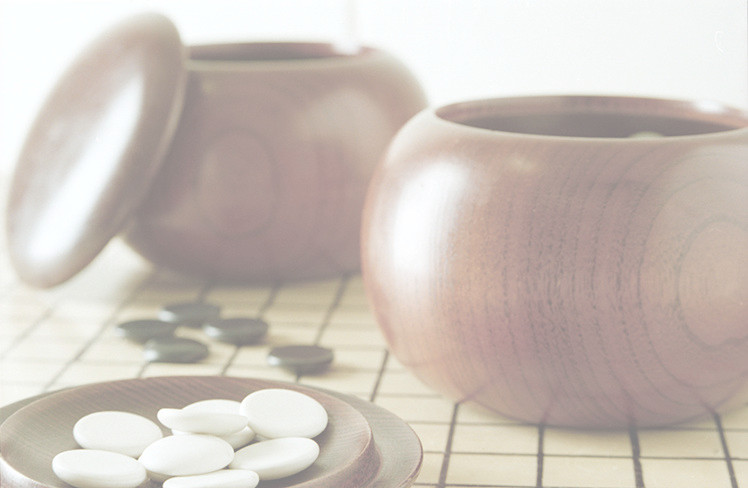
\includegraphics[width=\paperwidth,height=\paperheight]{images/bowls_board_faded.jpg}}
\frame{\titlepage}
}

\frame{\frametitle{Was ist Go?}
  \begin{itemize}
    \item Brettspiel für 2 Personen
    \item vor min. 2500 Jahren im antiken China erfunden
    \item Spielbrett: Gittermuster, auf Schnittpunkte werden Steine gesetzt
    \item Ziel: am Ende mehr als die Hälfte des Bretts zu besitzen
  \end{itemize}
  \vspace{0.1cm}
  \noindent\makebox[\textwidth]{
  \hspace{-1cm}
  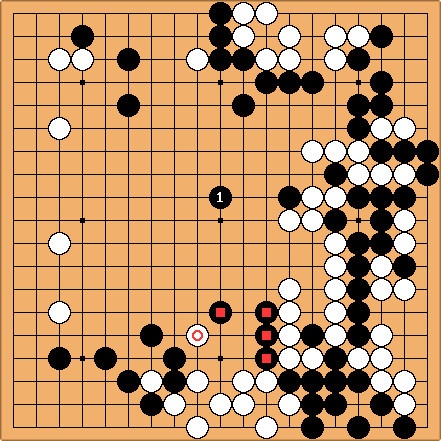
\includegraphics[height=4.5cm]{images/go_example.jpg}
  }
}

\frame{\frametitle{Spielregeln}
  \begin{enumerate}
    \item Spieler machen abwechselnd einen Zug (Schwarz beginnt)
    \item Zug: Setzen oder passen (nichts tun, Gegner an der Reihe)
    \item Setzen: Stein auf freien Punkt, zuerst gegnerische Ketten entfernen,
          dann eigene Ketten entfernen
    \item Kette wird entfernt, falls sie keine Freiheiten hat
    \item Freiheiten einer Kette: freie Punkte, die $\leftrightarrow \updownarrow$ an einen Stein der Kette
           angrenzen
    \item Setzen nicht erlaubt, falls es zu Zyklus führt
    \item beide Spieler passen hintereinander $\Rightarrow$ Auszählung
    \item Punkte pro Spieler: Anzahl Steine am Brett plus Gebiet
    \item Gebiet eines Spielers: freie Punkte, von denen man via $\leftrightarrow \updownarrow$  zur
          Farbe des Spielers kommt, nicht aber zur gegnerischen
    \item Spieler mit mehr Punkten gewinnt
  \end{enumerate}
}

\frame{\frametitle{Spielregeln erklärt}
  \begin{itemize}
    \item Schlagen 1
    \vspace{0.1cm}
    \noindent\makebox[\textwidth]{
    \hspace{-5.5cm}
    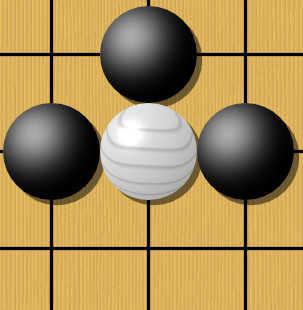
\includegraphics[height=3cm]{images/rules_capture1.jpg}
    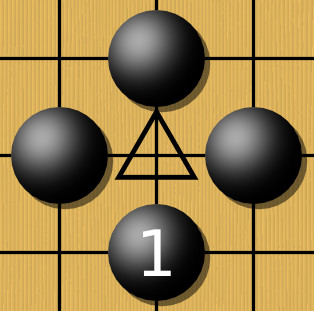
\includegraphics[height=3cm]{images/rules_capture2.jpg}
    }
    
    \item Schlagen 2
    \vspace{0.1cm}
    \noindent\makebox[\textwidth]{
    \hspace{-5.5cm}
    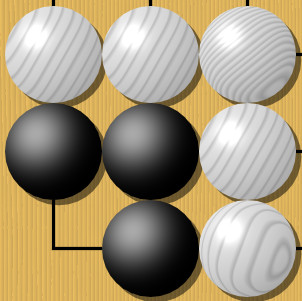
\includegraphics[height=3cm]{images/rules_capture3.jpg}
    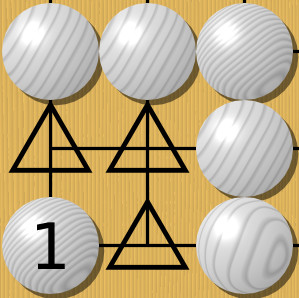
\includegraphics[height=3cm]{images/rules_capture4.jpg}
    }
  \end{itemize}
}

\frame{\frametitle{Spielregeln erklärt}
  \begin{itemize}
    \item Ko
    
    \vspace{0.1cm}
    \noindent\makebox[\textwidth]{
    \hspace{-5.5cm}
    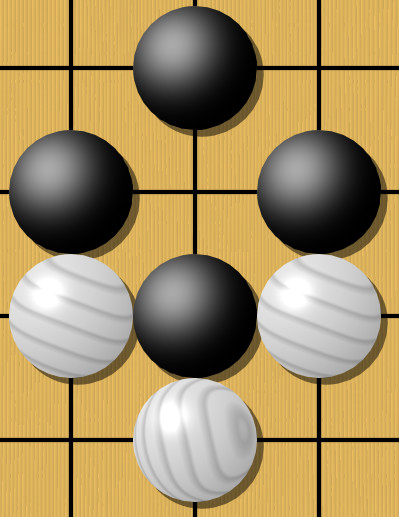
\includegraphics[height=2.5cm]{images/rules_ko1.jpg}
    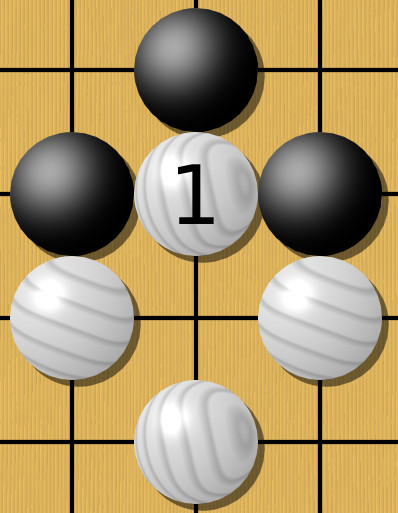
\includegraphics[height=2.5cm]{images/rules_ko2.jpg}
    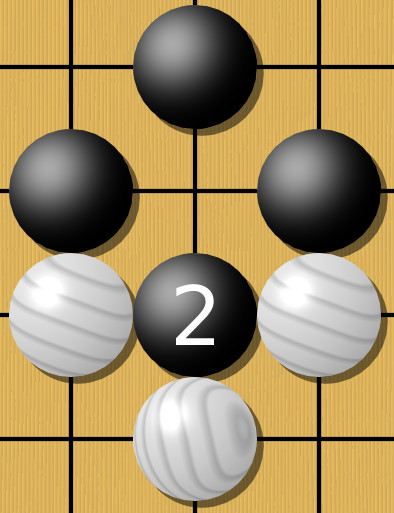
\includegraphics[height=2.5cm]{images/rules_ko3.jpg}
    }
    
    \item Auszählung
    \vspace{0.1cm}
    \noindent\makebox[\textwidth]{
    \hspace{-7.5cm}
    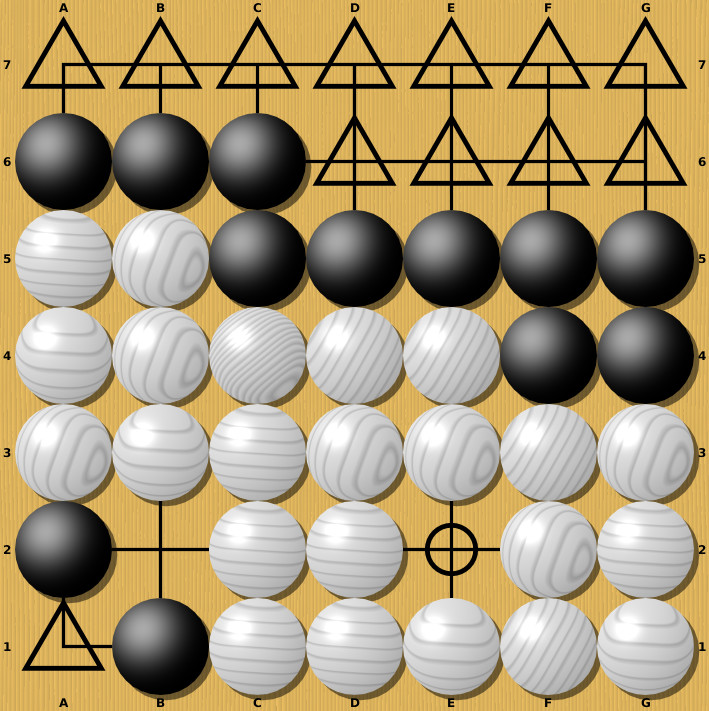
\includegraphics[height=4cm]{images/rules_scoring.jpg}
    }
  \end{itemize}
}

\frame{\frametitle{Taktiken / Motive}
  \begin{enumerate}
    \item Regel 1
  \end{enumerate}
}

\frame{\frametitle{Strategie: Leben und Tod}
  \begin{enumerate}
    \item Regel 1
  \end{enumerate}
}

\frame{\frametitle{Strategie: Balance halten}
  \begin{enumerate}
    \item Regel 1
  \end{enumerate}
}

\frame{\frametitle{Strategie: Langfristig planen}
  \begin{enumerate}
    \item Regel 1
  \end{enumerate}
}

\frame{\frametitle{Warum sollte man Go (nicht) spielen?}
  \begin{enumerate}
    \item Regel 1
  \end{enumerate}
}

\frame{\frametitle{Bezug zur Informatik}
  \begin{enumerate}
    \item Regel 1
  \end{enumerate}
}

\frame{\frametitle{Spielstärke / Handicap}
  \begin{enumerate}
    \item Regel 1
  \end{enumerate}
}


\end{document}
